\section{Genetic Operators}\label{sec:genetic_operators}
Similar to the genetic programming approach that did not incorporate modularization, the genetic operators used for this assignment included reproduction, crossover and mutation. Reproduction followed the textbook definition \cite{koza2005genetic} in that selected individuals were copied to the new population as is. Mutation consisted of selecting a tree from the selected individual; then, selecting a random node in that tree; and, finally, replacing the subtree rooted at that node in its entirety by a randomly-generated tree. Crossover selects the same tree from each of 2 selected individuals; then, a node is selected in each tree; and, finally, the two subtrees rooted at those nodes are swapped.

In terms of probabilities associated with genetic operators, the same probabilities as the approach that did not incorporate modularization were used. Specifically, the probability for crossover was 0.8, the probability for mutation was 0.1 and the probability for mutation was also 0.1. In addition, when applying operators decisions must be made regarding whether to select internal or leaf nodes. The probability for selecting a leaf node was chosen as 0.1 whereas the probability for selecting an internal node was chosen as 0.9. Finally, a maximum tree depth of 16 was applied as a constraint to the individuals of a new population. In the case of crossover and mutation, the operators would try to produce a valid individual up to 10 times before proceeding to the application of the next operator.

With the selection methods and genetic operators having been identified, figure \ref{fig:breeding_pipeline} depicts the entire breeding pipeline for generating a new population from an existing population.

\begin{figure}[H]
\centering
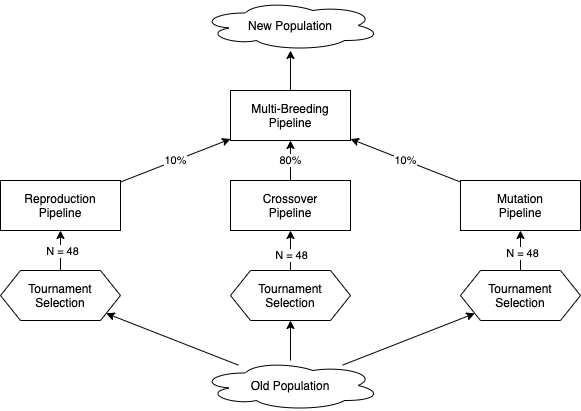
\includegraphics[width=\textwidth]{report/05_genetic_operators/breeding_pipeline.png}
\caption{Breeding Pipeline}
\label{fig:breeding_pipeline}
\end{figure}